\documentclass{report}

\input{~/dev/latex/template/preamble.tex}
\input{~/dev/latex/template/macros.tex}

\title{\Huge{}}
\author{\huge{Nathan Warner}}
\date{\huge{}}
\pagestyle{fancy}
\fancyhf{}
\lhead{Warner \thepage}
\rhead{}
% \lhead{\leftmark}
\cfoot{\thepage}
%\setborder
% \usepackage[default]{sourcecodepro}
% \usepackage[T1]{fontenc}

\begin{document}
    % \maketitle
        \begin{titlepage}
       \begin{center}
           \vspace*{1cm}
    
           \textbf{C++} \\
           From control structures  \\ through objects
    
           \vspace{0.5cm}
            
                
           \vspace{1.5cm}
    
           \textbf{Nathan Warner}
    
           \vfill
                
                
           \vspace{0.8cm}
         
           
\includegraphics[width=0.4\textwidth]{~/niu/seal.png}
                
           Computer Science \\
           Northern Illinois University\\
           September 1, 2023 \\
           United States\\
           
                
       \end{center}
    \end{titlepage}
    \tableofcontents
    \pagebreak \bigbreak \noindent
    \begin{center}
        \begin{Huge}
           \textbf{Preface} 
        \end{Huge}
    \end{center}
    \bigbreak \noindent 
    \sepline
    \bigbreak \noindent 
    \href{file:///home/datura/Downloads/Starting%20Out%20With%20C++%20From%20Control%20Structures%20Through%20Objects%208th%20Edition.pdf}{(click) ->}
    \href{file:///home/datura/Downloads/Starting%20Out%20With%20C++%20From%20Control%20Structures%20Through%20Objects%208th%20Edition.pdf}{(click)}
    \bigbreak \noindent 
    This document serves as a supplementary guide to \textit{C++ from Control Structures Through Objects by Tony Gaddis}. While the original text is geared towards beginners, this guide aims to assist those who already have programming experience, possibly in other languages.
    \bigbreak \noindent 
    To streamline the content and focus on aspects that are unique or nuanced in C++, this guide omits Chapters I and II of the original text. Instead, you will find a concise overview of the following foundational topics:
    \begin{itemize}
        \item Language Features
        \item The complier
        \item Boilerplate Code Structure
        \item Commenting Practices
        \item Data Types, Modifiers, Qualifiers, and Inference
        \item Type introspection
        \item Operators and Special Symbols
        \item The Using Directive
        \item Scope 
        \item Preprocessor Directives
        \item Standard Input/Output Techniques
    \end{itemize}
    \bigbreak \noindent
    Please note that basic elements like variables and arithmetic operations are not covered in this guide, under the assumption that readers are already familiar with these core computing concepts.

    %
    % This document will contain information found in \textit{C++ from control structures through objects by Tony Gaddis}. Although, this document will \textbf{not} be catered towards a beginning programmer, it is designed for those who may have experience in other languages. For this reason, this document will be omitting chapters I and II. In their place, there will  be a brief rundown on topics such as:
    % \begin{itemize}
    %     \item Boilerplate program
    %     \item Comments
    %     \item Includes
    %     \item Data types and modifiers
    %     \item Determine size of data types
    %     \item Symbols
    %     \item Input/Output
    %     \item scope
    % \end{itemize}
    % \bigbreak \noindent 
    % As an additional note, there \textbf{will not} be a section regarding variables, assignment statements, and arithemetic operations, as these are trivial to anyone familiar with concepts of computing.
    
    \pagebreak \bigbreak \noindent 
    \vspace{2.2in} \\
    \begin{Huge}
        \textbf{C++ from control \\ structures through objects}
    \end{Huge}
    \bigbreak \noindent 
    \sepline
    \bigbreak \noindent 
    \section{\LARGE The C++ Language}
    \bigbreak \noindent 
    C++ is a high-level, general-purpose programming language that was developed as an extension of the C programming language. Created by Bjarne Stroustrup, the first version was released in 1985. C++ is known for providing both high- and low-level programming capabilities. It is widely used for developing system software, application software, real-time systems, device drivers, embedded systems, high-performance servers, and client applications, among other things. C++ is praised for its performance and it's used for system/software development and in other fields, including real-time systems, robotics, and scientific computing.
    \bigbreak \noindent 
    \subsection{Key Features}
    \bigbreak \noindent 
    \begin{itemize}
        \item \textbf{Object-Oriented:} C++ supports Object-Oriented Programming (OOP), which allows for better organization and more reusable code. Concepts like inheritance, polymorphism, and encapsulation are available.
        \item \textbf{Procedural:} While C++ supports OOP, it also allows procedural programming, just like its predecessor C. This makes it easier to migrate code from C to C++.
        \item \textbf{Low-level Memory Access:} Like C, C++ allows for low-level memory access using pointers. This is crucial for system-level tasks.
        \item \textbf{STL (Standard Template Library):} C++ comes with a rich set of libraries that include pre-built functions and data types for a variety of common programming tasks, from handling strings to performing complex data manipulations.
        \item \textbf{Strongly Typed:} C++ has a strong type system to prevent unintended operations, although it does provide facilities to bypass this.
        \item \textbf{Performance:} One of the most significant advantages of C++ is its performance, which is close to the hardware level, making it suitable for high-performance applications.
        \item \textbf{Multiple Paradigms:} In addition to procedural and object-oriented programming, C++ also supports functional programming paradigms.
    \end{itemize}

    \pagebreak \bigbreak \noindent 
    \section{\LARGE The Compiler}
    \bigbreak \noindent 
    Unlike interpreted languages like Python or JS, C++ is a compiled language. The C++ compiler is a toolchain that takes C++ source code files and transforms them into executable files that a computer can run. The process involves several stages to get from human-readable C++ code to machine code that a CPU can execute.
    \bigbreak \noindent 
    Here's a general breakdown of the C++ compilation process:
    \bigbreak \noindent 
    \subsection{Preprocessing}
    \bigbreak \noindent 
    In this stage, the \textbf{preprocessor} takes care of directives like \#include, \#define, and \#ifdef. It replaces macros with their actual values and includes header files into the source code. The output of this stage is an expanded source code file.
    \begin{itemize}
        \item \textbf{Macro Replacement:} Replace macros with their respective values.
        \item \textbf{File Inclusion:} Include header files specified by \#include directives.
        \item \textbf{Conditional Compilation:} Code between \#ifdef and \#endif (or related preprocessor conditionals) is included or excluded based on the condition.
    \end{itemize}

    \bigbreak \noindent 
    \subsection{Lexical Analysis}
    \bigbreak \noindent 
    The expanded source code is then tokenized into a sequence of tokens (keywords, symbols, identifiers, etc.). This stage is known as lexical analysis or scanning. The lexer converts the character sequence of the program into a sequence of lexical tokens.

    \bigbreak \noindent 
    \subsection{Syntax Analysis}
    \bigbreak \noindent 
    The sequence of tokens is then parsed into a syntax tree based on the grammar rules of the C++ language. This stage is known as syntax analysis or parsing. The parser checks whether the code follows the syntax rules of C++ and constructs a syntax tree which is used in the subsequent stages of the compiler.

    \bigbreak \noindent 
    \subsection{Semantic Analysis}
    \bigbreak \noindent 
    Semantic rules like type-checking, scope resolution, and other language-specific constraints are verified at this stage. For example, it ensures that variables are declared before use, that functions are called with the correct number and types of arguments, etc.

    \bigbreak \noindent 
    \subsection{Intermediate Code Generation}
    \bigbreak \noindent 
    The syntax tree or another intermediate form is then converted into an intermediate representation (IR) of the code. This is often a lower-level form of the code that is easier to optimize.

    \bigbreak \noindent 
    \subsection{Code Optimization}
    \bigbreak \noindent 
    The compiler attempts to improve the intermediate code so that it runs faster and/or takes up less space. This can involve removing unnecessary instructions, simplifying calculations, etc.

    \bigbreak \noindent 
    \subsection{Code Generation}
    \bigbreak \noindent 
    The optimized intermediate representation is then translated into assembly code for the target platform. The assembly code is specific to the computer architecture and can be assembled into machine code.

    \bigbreak \noindent 
    \subsection{Assembling}
    \bigbreak \noindent 
    The assembly code is then processed by an assembler to produce object code, which consists of machine-level instructions.

    \bigbreak \noindent 
    \subsection{Linking}
    \bigbreak \noindent 
    Finally, the object code is linked with other object files and libraries to produce the final executable. The linker resolves all external symbols, combines different pieces of code, and arranges them in memory to create a standalone executable.

    \bigbreak \noindent 
    \subsection{Complier Options}
    \bigbreak \noindent 
    For linux users that are not using IDES, we are free to choose which complier to use when building C++ code. The most common compliers are:
    \begin{itemize}
        \item \textbf{g++} (GCC (GNU Compiler Collection)): GCC is the de facto standard compiler for Linux. It supports multiple programming languages, but you'll most commonly use g++ for compiling C++ code.
            \begin{itemize}
                \item \textbf{Compile a program:} g++ source.cpp -o output
                \item \textbf{Compile and link multiple files:} g++ source1.cpp source2.cpp -o output
                \item \textbf{Use C++11 or later standards:} g++ -std=c++11 source.cpp -o output
            \end{itemize}
        \item \textbf{Clang:} Clang is known for its fast compilation and excellent diagnostics. It's part of the LLVM project and is fully compatible with GCC.
            \begin{itemize}
                \item \textbf{Compile a program:} clang++ source.cpp -o output
                \item \textbf{Compile and link multiple files:} clang++ source1.cpp source2.cpp -o output
                \item \textbf{Use C++11 or later standards:} clang++ -std=c++11 source.cpp -o output
            \end{itemize}
        \item \textbf{Intel C++ Compiler}: The Intel C++ Compiler (icpc) is focused on performance and is optimized for Intel processors, although it can also generate code for AMD processors.
            \begin{itemize}
                \item \textbf{Compile a program:} icpc source.cpp -o output
                \item \textbf{Compile and link multiple files:} icpc source1.cpp source2.cpp -o output
                \item \textbf{Use C++11 or later standards:} icpc -std=c++11 source.cpp -o output
            \end{itemize}
    \end{itemize}

    \bigbreak \noindent 
    \subsection{Header Files}
    Header files are generally not included in the command line arguments when compiling. However, we can specify to the complier where to look for them:
    \bigbreak \noindent 
    \sepline
    \begin{minted}{bash}
g++ -I path/to/headerfiles/ main.cpp -o main
g++ -isystem path/to/system/headerfiles/ main.cpp -o main
    \end{minted}
    \sepline
















    \pagebreak \bigbreak \noindent 
    \section{\LARGE Preliminaries: A Quick Tour of C++ Fundamentals}
    \bigbreak \noindent 
    \subsection{Boilerplate}
    \bigbreak \noindent 
    We will begin with a examination of the boilerplate c++ code that will serve as an entry to most programs.
    \sepline
    \begin{minted}[linenos]{cpp}
#include <iostream>
#include <iomanip>

int main(int argc, char argv[]){

    return 0
}
    \end{minted}
    \sepline
    \bigbreak \noindent 
    Every C++ program has a primary function that must be named \textbf{main} . The main function serves as the starting point for program execution. It usually controls program execution by directing the calls to other functions in the program.
    \bigbreak \noindent 
    The includes at the top of the program are common in a c++ program, they are \textit{iostream} and \textit{iomanip}. These library's allow us to recieve input via the input stream, as well as to output information  via the output stream. Whereas \textit{iomanip} allows us to preform varies manipulations on such streams.
    \bigbreak \noindent 
    \nt{return 0 is important in our main function, this is because the \textit{int} you see in front of \textit{main} declares which data type the function must return. Note that you may also see \textbf{EXIT\_SUCCESS} or \textbf{EXIT\_FAILURE}. These, along with any other integer values are suitable return types for the main function.}

    \bigbreak \noindent 
    \subsection{The main function}
    \bigbreak \noindent 
    The main() function serves as the entry point for a C++ program. When you execute a compiled C++ program, the operating system transfers control to this function, effectively kicking off the execution of your code.
    \bigbreak \noindent 
    In C++, you generally cannot execute code like std::cout $<<$ "Hello, world!"; outside of a function body. Code execution starts from the main() function, and any executable code outside of a function is not valid C++ syntax. However you can declare and initialize variables, functions etc. Note that if you try to assign a variable you will get an error. 

    \bigbreak \noindent 
    \subsection{Comments}
    In order to display comments in our C++ program, we use // (double forward slashes)
    \bigbreak \noindent 
    \sepline
    \begin{minted}[linenos]{cpp}
#include <iostream> 
#include <iomanip>

int main() {
    // This is a comment
    /* This is a Multi Line Comment */

    return EXIT_SUCCESS;
}
    \end{minted}
    \sepline

    \pagebreak \bigbreak \noindent 
    \subsection{Data Types, Modifiers, Qualifiers, Inference}
    \begin{minipage}[t]{0.47\textwidth}
    \textbf{Integer type}
    \begin{itemize}
        \item \textbf{int} (4 bytes on most systems)
        \item \textbf{long} (4 or 8 bytes depending on system)
        \item \textbf{long long} (At least 8 bytes)
    \end{itemize}
\end{minipage}
\begin{minipage}[t]{0.47\textwidth}
    \textbf{Character Types}
    \begin{itemize}
        \item char (1 byte)
        \item wchar\_t (2 or 4 bytes)
        \item char16\_t (2 bytes)
        \item char32\_t (4 bytes)
    \end{itemize}
\end{minipage}
\bigbreak \noindent 
\begin{minipage}[t]{0.47\textwidth}
    \textbf{Floating point types}
    \begin{itemize}
        \item float (4 bytes) (always signed)
        \item double (8 bytes) (always signed)
        \item long double (8, 12, or 16 bytes) (always signed)
    \end{itemize}
\end{minipage}
\begin{minipage}[t]{0.47\textwidth}
    \textbf{Boolean Type}
    \begin{itemize}
        \item bool (1 byte)
    \end{itemize}
\end{minipage}
\bigbreak \noindent \bigbreak \noindent 
\begin{minipage}{0.47\textwidth}
    \textbf{Void type}
    \begin{itemize}
        \item void (No storage)
    \end{itemize}
\end{minipage}
\begin{minipage}{0.47\textwidth}
    \textbf{String type}
    \begin{itemize}
        \item std::string (Depends on length) \footnote{must include <string>}
    \end{itemize}
\end{minipage}
\bigbreak \noindent \bigbreak \noindent 
\begin{minipage}[t]{0.47\textwidth}
    \textbf{C Modifiers for int, bool and char}
    \begin{itemize}
        \item unsigned (Same as base type)
        \item signed  (Same as base type)
        \item short (Usually 2 bytes)
        \item long (4 or 8 bytes)
        \item long long (At least 8 bytes)
    \end{itemize}
\end{minipage}
\begin{minipage}[t]{0.47\textwidth}
    \textbf{Fixed-Width Integer Types: (defined in $<$cstdint$>$)}
    \begin{itemize}
        \item int8\_t (1 byte) \quad \quad \textbullet uint8\_t (1 byte)
        \item int16\_t (2 bytes) \quad \textbullet uint16\_t (2 bytes)
        \item int32\_t (4 bytes) \quad \textbullet uint32\_t (4 bytes)
        \item int64\_t (8 bytes) \quad \textbullet uint64\_t (8 bytes)
    \end{itemize}
\end{minipage}
\bigbreak \noindent \bigbreak \noindent 
\begin{minipage}[t]{0.47\textwidth}
    \textbf{Type Qualifiers:}
    \begin{itemize}
        \item const (No additional storage)
        \item volatile (No additional storage)
    \end{itemize}
\end{minipage}
\begin{minipage}[t]{0.47\textwidth}
    \textbf{Inference}
    \begin{itemize}
        \item auto (Depends on the type it infers)
        \item decltype (Depends on the type it infers)
    \end{itemize}
\end{minipage}

    \pagebreak \bigbreak \noindent 
    \subsection{Creating strings without the STL}
    To create a string \textbf{without} using the C++ standard library (STL), we can create an array of characters. For this we have two options.
    \bigbreak \noindent 
    \sepline
    \begin{minted}[linenos]{cpp}
int main() {

    // Option I
    char mystring[] = "hello world";

    // Option II
    const char* mystring = "Hello World";
    return 0;
}
    \end{minted}
    \sepline
    \bigbreak \noindent 
    Note regarding the first option: simply declaring mystring without any sort of initialization will through an error. This is due to the way arrays behave in c++, more on this later.
    \bigbreak \noindent 
    For the second option, we declare a pointer of characters. Note that although it is declared constant, it is legal to change the value of mystring. We can't change the characters that are pointed at, but we can change the pointer itself.
    \bigbreak \noindent 
    Furthermore, It is worth pointing out that there is a third way of making a string without use of the STL, it is as follows.
    \bigbreak \noindent 
    \sepline
    \begin{minted}[linenos]{cpp}
#include <iostream>

int main(int argc, char agrv[]){

    char const* mystring = "Hello world";

    return 0;
}
    \end{minted}
    \sepline
    \bigbreak \noindent 
    The const modifier in C++ binds to the element that is immediately to its left, except when there is nothing to its left, in which case it binds to the element immediately to its right.
    \bigbreak \noindent 
    \nt{Usage of the asterisk will be discussed in a later section. This concept is known as the "pointer"}


    \pagebreak \bigbreak \noindent 
    \subsection{Retrieve size}
    \bigbreak \noindent 
    To retrieve the size of a variable or data type we can use the sizeof() function.
    \bigbreak \noindent 
    \sepline
    \begin{minted}[linenos]{cpp}
#include <iostream>
using std::cout;
using std::endl;

int main() {
    int a = 12;
    cout << sizeof(a) << endl;

    return 0;
}
    \end{minted}
    \sepline

    \bigbreak \noindent \bigbreak \noindent 
    \subsection{Retrieve type}
    \bigbreak \noindent 
    To retrieve the type of a variable we can use the typeid().name() function. Note that this function is part of the <typeinfo> library
    \bigbreak \noindent 
    \sepline
    \begin{minted}[linenos]{cpp}
#include <iostream>
#include <typeinfo>
using std::cout;
using std::endl;

int main(){

    int a = 12;

    cout << typeid(a).name() << endl;

    return 0
}
    \end{minted}
    \sepline
    \pagebreak \bigbreak \noindent 
    \subsection{Exponential Notation}
    \bigbreak \noindent 
    In C++, you can use exponential notation to represent floating-point numbers. This is particularly useful when you're dealing with very large or very small numbers. In exponential notation, a floating-point number is represented as a base and an exponent, often separated by the letter e or E.
    \bigbreak \noindent 
    \sepline
    \begin{minted}[linenos]{cpp}
#include <iostream>

int main(int argc, char argv[]){
    double num1 = 1.23e4;
    double num2 = 1.23e-4;
    double num3 = 5e6;
    double num4 = 5e+6; // The same as the previous example (num3)

    // Outputting the numbers
    std::cout << "num1: " << num1 << std::endl;  // Output should be 12300
    std::cout << "num2: " << num2 << std::endl;  // Output should be 0.000123
    std::cout << "num3: " << num3 << std::endl;  // Output should be 5000000
    return 0;
}
    \end{minted}
    \sepline
    \bigbreak \noindent 
    \nt{Note that while you can use exponential notation for readability and convenience, the variables themselves will store the actual values. For example, num1 will actually store 12300.0, not 1.23e4.}
    \bigbreak \noindent 
%     You can also use exponential notation when initializing float and long double variables:
%     \bigbreak \noindent 
%     \sepline
%     \begin{minted}[linenos]{cpp}
% #include <iostream>
%
% int main(int argc, char argv[]){
%     float a = 3.14e2f;          // 'f' suffix for float
%     long double b = 2.71e3l;    // 'l' suffix for long double
%
%     // or
%
%     float a = 3.14e2F;          // 'f' suffix for float
%     long double b = 2.71e3L;    // 'l' suffix for long double
%
%     return 0;
% }
%     \end{minted}
%     \sepline

    \bigbreak \noindent   
    \subsection{Type Conversion}
    \textbf{Concept.} When an operator's operands are of different data types, C++ will automatically convert them to the same data type. C++ follows a set of rules when performing mathematical operations on variables of different data types.
    \bigbreak \noindent 
    \textbf{Data Type Ranking:}
    \begin{enumerate}
        \item long double
        \item double 
        \item float
        \item unsigned long long int
        \item long long int
        \item unsigned long int
        \item long int
        \item unsigned int
        \item int
    \end{enumerate}
    \bigbreak \noindent 
    \textbf{Rule 1:} Chars, shorts, and unsigned shorts are automatically promoted to int.
    \bigbreak \noindent 
    \textbf{Rule 2:} The lower-ranking value is promoted to the type of the higher ranking value.


    \bigbreak \noindent
    \subsection{Integer Division}
    \bigbreak \noindent 
    \textbf{Concept.} When you divide an integer by another integer in c++, the result is always an integer.

    \bigbreak \noindent 
    \subsection{Overflow/Underflow}
    \bigbreak \noindent 
    \textbf{Concept.} When a variable is assigned a value that is too large or too small in range for that variable's data type, the variable overflows or underflows. Ty
    \bigbreak \noindent 
    
    \bigbreak \noindent 
    \subsection{Type Casting}
    \bigbreak \noindent 
    \textbf{Concept.} Type Casting allows you to perform manual data type conversion. The general syntax of a type cast expression is:
    \bigbreak \noindent 
    \sepline
    \begin{minted}[linenos]{cpp}
static_cast<Type>(value)
    \end{minted}
    \sepline
    \bigbreak \noindent 
    Consider the example
    \smallbreak \noindent
    \sepline
    \begin{minted}[linenos]{cpp}
#include <iostream>

int main(int argc, char argv[]){
    int a = 12.12;
    a = static_cast<float>(a);

    return 0;
}
    \end{minted}
    \sepline
    \bigbreak \noindent 
    Even though you are casting a to a float, the variable $a$ stays as an integer because you are assigning the result back into $a$, which was originally declared as an integer. In C++, you can't change the data type of a variable once it's declared; you can only temporarily alter how it behaves through casting.

    \bigbreak \noindent 
    \subsection{C-style Casts}
    \bigbreak \noindent 
    It is worth noting that static\_cast is not our only option. There is the standard C-style cast:
    \bigbreak \noindent 
    \sepline
    \begin{minted}[linenos]{cpp}
float a = 12.2;
cout << (int) a;
    \end{minted}
    \sepline
    % \bigbreak \noindent 
    % And we also have:
    % \begin{itemize}
    %     \item \textbf{const\_cast:} This type of cast adds or removes the const modifier from a variable.
    %     \item \textbf{reinterpret\_cast:}
    %     \item \textbf{dynamic\_cast:}
    % \end{itemize}
    




    \pagebreak \bigbreak \noindent 
    \subsection{The Using Directive}
    \bigbreak \noindent 
    The using namespace directive allows you to use names (variables, types, functions, etc.) from a particular namespace without prefixing them with the namespace name. For example:
    \bigbreak \noindent 
    \sepline
    \begin{minted}[linenos]{cpp}
#include <iostream>
#include <iomanip>
using namespace std;

int main(){
    cout << "Hello World" << endl;
    return 0;
}
    \end{minted}
    \sepline
    \bigbreak \noindent 
    Here, cout and endl are part of the std namespace, and the using statement allows us to use them without the std:: prefix. This is convenient but can lead to name clashes if multiple namespaces have elements with the same name. Instead we can do:
    \bigbreak \noindent 
    \sepline
    \begin{minted}[linenos]{cpp}
#include <iostream>
#include <iomanip>
using std::cout;
using std::endl;

int main(){
    cout << "Hello World" << endl;
    return 0;
}
    \end{minted}
    \sepline
    \bigbreak \noindent 
    We can also use this directive to create an alias for a type. This is especially useful for simplifying complex or templated types:
    \bigbreak \noindent 
    \sepline
    \begin{minted}[linenos]{cpp}
#include <iostream>
#include <iomanip>
using std::cout;
using std::endl;

using myint = int;

int main() {
    
    myint a = 12;
    cout << a << endl;

    return EXIT_SUCCESS;
}
    \end{minted}
    \sepline

    \pagebreak \bigbreak \noindent 
    \subsection{Variable Declaration}
    \bigbreak \noindent 
    Declaring a variable means telling the compiler about its name and type, but not necessarily assigning a value to it. At the time of declaration, memory is allocated for the variable. You may or may not initialize it immediately. Here are some examples:
    \bigbreak \noindent 
    \sepline
    \begin{minted}[linenos]{cpp}
int a;              // Declaration without initialization
float b;            // Another declaration without initialization
char c = 'A';       // Declaration with initialization
double d = 3.14;    // Another declaration with initialization
std::string str;    // Declaration without initialization
    \end{minted}
    \sepline
    \bigbreak \noindent 
    Note that variables of built-in types declared without initialization will have an undefined value in C++ until you explicitly assign a value to them. However, global and static variables are automatically initialized to zero if you do not explicitly initialize them.

    \bigbreak \noindent 
    \subsection{Multiple Declaration}
    \bigbreak \noindent 
    In c++, we can declare multiple variables on a single line:
    \bigbreak \noindent 
    \sepline
    \begin{minted}[linenos]{cpp}
int a,b,c
    \end{minted}
    \sepline

    \bigbreak \noindent 
    \subsection{Initialization}
    \bigbreak \noindent 
    We can also combine declaration and assignment together:
    \bigbreak \noindent 
    \sepline
    \begin{minted}[linenos]{cpp}
int a = 12;
    \end{minted}
    \sepline

    \bigbreak \noindent 
    \subsection{Multiple Initialization}
    \bigbreak \noindent 
    We can declare and assign multiple variables on a single line with:
    \bigbreak \noindent 
    \sepline
    \begin{minted}[linenos]{cpp}
int a = 5, b = 10, c = 15;
    \end{minted}
    \sepline

    \bigbreak \noindent 
    \subsection{Direct Initialization}
    \bigbreak \noindent 
    \sepline
    \begin{minted}[linenos]{cpp}
int a(5);
    \end{minted}
    \sepline
    \bigbreak \noindent 
    In this case, the variable a is directly initialized with the value 5 using parentheses. This is known as "direct initialization." Direct initialization is generally straightforward and efficient.

    \bigbreak \noindent 
    \subsection{List Initialization}
    \bigbreak \noindent 
    \sepline
    \begin{minted}[linenos]{cpp}
int a{5};
    \end{minted}
    \sepline
    \bigbreak \noindent 
    Here, the variable b is initialized with the value 10 using curly braces. This is called "list initialization" or "uniform initialization" and is available starting with C++11. One of its advantages is that it prevents narrowing conversions (e.g., from double to int without a cast).
    \bigbreak \noindent 
    List initialization has the benefit of disallowing narrowing conversions, making it somewhat safer. For example, int x{3.14}; would cause a compiler error, while int x = 3.14; would compile with a possible warning, depending on the compiler settings.

    \bigbreak \noindent 
    \subsection{Copy Initialization}
    \bigbreak \noindent 
    \sepline
    \begin{minted}[linenos]{cpp}
int a = 5;
    \end{minted}
    \sepline
    \bigbreak \noindent 
    In this style, known as "copy initialization," the variable c is initialized with the value 15 using the = operator. This is one of the most commonly used forms of initialization.



    \bigbreak \noindent 
    \subsection{Assignment}
    \bigbreak \noindent 
    Assignment refers to the action of storing a value in a variable that has already been declared. This is done using the assignment operator =.
    \bigbreak \noindent 
    \sepline
    \begin{minted}[linenos]{cpp}
a = 10;            // Assignment
b = 3.14f;         // Another assignment
c = 'B';           // Another assignment
d = 2.71;          // Another assignment
str = "Hello";     // Another assignment
    \end{minted}
    \sepline
    \bigbreak \noindent 
    \subsection{Multiple Assignment}
    \bigbreak \noindent 
    We can assign multiple variables on a single line:
    \bigbreak \noindent 
    \sepline
    \begin{minted}[linenos]{cpp}
a = 5, b = 10, c = 15;
    \end{minted}
    \sepline

    \pagebreak \bigbreak \noindent 
    \section{\LARGE Symbols}
    \bigbreak \noindent 
    \begin{minipage}[t]{0.47\textwidth}
        \subsection{Parentheses}
        \bigbreak \noindent 
        Parentheses are used for several purposes:
        \begin{itemize}
            \item Function calls: myFunction(arg1, arg2)
            \item Operator precedence: (a + b) * c
            \item Casting: (int) myDouble
            \item Control statements: if (condition) { ... }
        \end{itemize}
    \end{minipage}
    \begin{minipage}[t]{0.47\textwidth}
    \subsection{Brackets}
    \bigbreak \noindent 
    Square brackets are generally used for:
    \begin{itemize}
        \item Array indexing: myArray[2] = 5;
        \item Vector and other container types also use this syntax for element access.
    \end{itemize}
    \end{minipage}
    \bigbreak \noindent \bigbreak \noindent 
    \begin{minipage}[t]{0.47\textwidth}
    \subsection{Braces}
    \bigbreak \noindent 
    Braces Braces define a scope and are \\ commonly used for:
    \begin{itemize}
        \item Enclosing the bodies of functions, loops, and conditional statements.
        \item Initializer lists.
        \item Defining a struct or class.
    \end{itemize}
    %\caption{}
    %\label{fig:}
    \end{minipage}
    \begin{minipage}[t]{0.67\textwidth}
    \subsection{Angle Brackets}
    \bigbreak \noindent 
    Angel Brackets are used in:
    \begin{itemize}
        \item Template declaration and instantiation: std::vector$<$int$>$
        \item Shift operators: a $<<$ 2, b $>>$ 2
        \item Comparison: a $<$ b, a $>$ b
    \end{itemize}
    \end{minipage}
    \bigbreak \noindent \bigbreak \noindent
    \begin{minipage}[t]{0.47\textwidth}
    \subsection{Semi Colon}
    \bigbreak \noindent 
    Semi colons are used for:
    \begin{itemize}
        \item Terminate statements 
        \item Separate statements within a single line
        \item After class and struct definitions.
    \end{itemize}
    \end{minipage}
    \begin{minipage}[t]{0.47\textwidth}
    \subsection{Colon}
    \bigbreak \noindent 
    Colons are used for:
    \begin{itemize}
        \item Inheritance and interface implementation: class Derived : public Base { ... }
        \item Label declaration for goto statements.
        \item Range-based for loops (C++11 and above): for (auto i : vec)
        \item Bit fields in structs: struct S { unsigned int b : 3; };
        \item To initialize class member variables in constructor initializer lists.
    \end{itemize}
    \end{minipage}
    \bigbreak \noindent \bigbreak \noindent
    \begin{minipage}[t]{0.47\textwidth}
    \subsection{Comma}
    \bigbreak \noindent 
    Commas are used for:
    \begin{itemize}
        \item Separate function arguments
        \item Separate variables in a declaration: int a = 1, b = 2;
        \item Create a sequence point, executing left-hand expression before right-hand expression: a = (b++, b + 2);
    \end{itemize}
    \end{minipage}
    \begin{minipage}[t]{0.47\textwidth}
    \subsection{Ellipsis}
    \bigbreak \noindent 
    Ellipsis are used for:
    \begin{itemize}
        \item Variable number of function arguments (C-style): void myFunc(int x, ...)
    \end{itemize}
    %\caption{}
    %\label{fig:}
    \end{minipage}
    \bigbreak \noindent 
    \begin{minipage}[t]{0.47\textwidth}
        \subsection{Hash}
        \bigbreak \noindent 
        Hashes are used for preprocessor  directives
    \end{minipage}



    \pagebreak \bigbreak \noindent 
    \section{Preprocessor Directives}
    \bigbreak \noindent 
    C++ preprocessor directives are lines in your code that start with the hash symbol (\#). These directives are not C++ statements or expressions; instead, they are instructions to the preprocessor about how to treat the code. Here's an overview of some of the most commonly used preprocessor directives in C++:
    \bigbreak \noindent 
    \subsection{\#include}
    \bigbreak \noindent 
    Used to include the contents of a file within another file. This is commonly used for including standard library headers or user-defined header files.
    \bigbreak \noindent 
    \sepline
    \begin{minted}[linenos]{cpp}
#include <iostream>
#include "myheader.h"
    \end{minted}
    \sepline

    \bigbreak \noindent 
    \subsection{\#define}
    \bigbreak \noindent 
    Used for macro substitution. It can define both simple values and more complex macro functions.
    \bigbreak \noindent 
    \sepline
    \begin{minted}[linenos]{cpp}
#define PI 3.14159 // Defines PI as 3.14159.
#define SQUARE(x) ((x)*(x)) // Defines a macro that squares its argument.
    \end{minted}
    \sepline

    \bigbreak \noindent 
    \subsection{\#undef}
    \bigbreak \noindent 
    Undefines a preprocessor macro, making it possible to redefine it later.
    \bigbreak \noindent 
    \sepline
    \begin{minted}[linenos]{cpp}
#undef PI
    \end{minted}
    \sepline

    \bigbreak \noindent 
    \subsection{\#ifdef, \#ifndef, \#else, \#elif, \#endif}
    \bigbreak \noindent 
    These are used for conditional compilation.
    \bigbreak \noindent 
    \sepline
    \begin{minted}[linenos]{cpp}
#ifdef DEBUG // Compiles the following code only if DEBUG is defined.
#ifndef DEBUG // Compiles the following code only if DEBUG is not defined.
#else // Provides an alternative if the preceding #ifdef or #ifndef fails.
#elif // Like else if in standard C++, allows chaining conditions.
#endif // Ends a conditional compilation block.
    \end{minted}
    \sepline

    \bigbreak \noindent 
    \subsection{\#if}
    \bigbreak \noindent 
    Like \#ifdef, but it allows for more complex expressions.
    \bigbreak \noindent 
    \sepline
    \begin{minted}[linenos]{cpp}
#if defined(DEBUG) && !defined(RELEASE) // Multiple conditions using logical operators.
    \end{minted}
    \sepline

    \bigbreak \noindent 
    \subsection{\#pragma}
    \bigbreak \noindent 
    Issues special commands to the compiler. These are compiler-specific and non-portable.
    \bigbreak \noindent 
    \sepline
    \begin{minted}[linenos]{cpp}
#pragma once 
/* Ensures that the header file is included only once during compilation. 
This is an alternative to the traditional include guard (#ifndef, #define, #endif). */
    \end{minted}
    \sepline

    \bigbreak \noindent 
    \subsection{\#error}
    \bigbreak \noindent 
    Generates a compile-time error with a message.
    \bigbreak \noindent 
    \sepline
    \begin{minted}[linenos]{cpp}
#error "Something went wrong" // Produces a compilation error with the given message.
    \end{minted}
    \sepline

    \bigbreak \noindent 
    \subsection{\#line}
    \bigbreak \noindent 
    Changes the line number and filename for error reporting and debugging.
    \bigbreak \noindent 
    \sepline
    \begin{minted}[linenos]{cpp}
#line 20 "myfile.cpp" // Sets the line number to 20 and the filename to "myfile.cpp".
    \end{minted}
    \sepline

    \pagebreak \bigbreak \noindent 
    \section{\LARGE Input/Output}
    \bigbreak \noindent 
    This section will discuss the input/output stream, and objects defined in the iostream and iomanip headers.
    \bigbreak \noindent 
    \subsection{iostream}
    \bigbreak \noindent 
    The $<$iostream$>$ header file in C++ defines classes that provide functionalities for basic input-output operations. These classes are part of the C++ Standard Library and offer a high-level interface for I/O. The primary classes defined by $<$iostream$>$ are:
    \begin{itemize}
        \item \textbf{istream:} Input Stream class. Objects of this class are used for input operations. The most commonly used object is cin.
        \item \textbf{ostream:} Output Stream class. Objects of this class are used for output operations. The most commonly used object is cout.
    \end{itemize}
    \bigbreak \noindent 
    \subsection{Output}
    \bigbreak \noindent 
    We can output data to the stream buffer with the cout object, here is an example:
    \bigbreak \noindent 
    \sepline
    \begin{minted}[linenos]{cpp}
#include <iostream>
using std::cout;
using std::endl;

int main(int argc, char argv[]){

    cout << "Hello World" << endl;

    return 0;
}
    \end{minted}
    \sepline
    \bigbreak \noindent 
    \subsection{Input}
    \bigbreak \noindent 
    We can read data from the input stream and store in a variable with the cin object, here is an example:
    \bigbreak \noindent 
    \sepline
    \begin{minted}[linenos]{cpp}
#include <iostream>
using std::cin;
using std::cout;
using std::endl;

int main(int argc, char argv[]){
    int a;
    cout << "Input: " << endl;
    cin >> a;
    return 0;
}

    \end{minted}
    \sepline

    \pagebreak \bigbreak \noindent 
    \subsection{IO Manipulators}
    \bigbreak \noindent 
    In C++, input/output (I/O) manipulators are objects that are used for controlling the formatting and behavior of streams. These manipulators allow you to change the way data is presented when outputting to a stream (like cout) or read when inputting from a stream (like cin).
    \bigbreak \noindent 
    Here are some common manipulators:
    \begin{itemize}
        \item \textbf{std::endl}:  Inserts a newline character into the output sequence os and flushes it \footnote{Defined in <ostream> which is included automatically with <iostream>}
            \smallbreak
            \sepline
            \begin{minted}[linenos]{cpp}
            std::cout << "Hello World" << std::endl;
            \end{minted}
            \sepline
        \item \textbf{std::flush}  Explicitly flushes the output buffer. \footnote{Refer to 1}
            \smallbreak
            \sepline
            \begin{minted}[linenos]{cpp}
            std::cout << "Hello World" << std::flush;
            \end{minted}
            \sepline
        \item \textbf{std::setw($n$)} Sets the field width for the next insertion operation. \footnote{Defined in <iomanip>}
            \smallbreak
            \sepline
            \begin{minted}[linenos]{cpp}
            std::cout << std::setw(10) << 77 << endl; 
            // Output will be "        77"
            \end{minted}
            \sepline
        \item \textbf{std::setfill(char)} Sets the fill character for the std::setw manipulator. \footnote{Refer to 3}
            \smallbreak
            \sepline
            \begin{minted}[linenos]{cpp}
            std::cout << std::setw(10) << std::setfill('_') << 77 << endl; 
            // Output will be "________77"
            \end{minted}
            \sepline

        \item \textbf{std::setprecision($n$)} Sets the decimal precision for floating-point output. $n$ should be  \\ one more than the required rounding, this is because $n$ specifys how many significant  \\ figures to include. Thus including any numbers before the decimal. \footnote{Refer to 3} \\
            \textbf{Note:} once specified setprecision will be persistent throughout the rest of the program. This is also true when used in conjunction with std::fixed

            \smallbreak
            \sepline
            \begin{minted}[linenos]{cpp}
            std::cout << std::setprecision(4) << 3.14159; // 3.142
            \end{minted}
            \sepline
            \pagebreak \bigbreak \noindent 
        \item \textbf{std::fixed}: Use fixed-point notation. Works in conjunction to setprecision, allowing \\ you to not have to account for digits before the decimal.  \footnote{Defined in <ios>, which is automatically included with <iostream>}
            \smallbreak
            \sepline
            \begin{minted}[linenos]{cpp}
            std::cout << std::fixed << std::setprecision(3) << 3.14159; 
            // 3.142
            \end{minted}
            \sepline
        \item \textbf{std::scientific:} Use scientific notation for floating-point numbers. \footnote{Refer to 6}
            \smallbreak
            \sepline
            \begin{minted}[linenos]{cpp}
            std::cout << std::scientific << 0.00000014159; 
            // 1.415900e-07 
            \end{minted}
            \sepline
        \item \textbf{std::skipws and std::noskipws:} These control whether leading whitespaces are \\ skipped when performing input operations. \footnote{Refer to 6}
            \smallbreak
            \sepline
            \begin{minted}[linenos]{cpp}
            char a,b;
            std::cin >> std::noskipws >> a >> b;
            \end{minted}
            \sepline
        \item \textbf{std::boolalpha and std::noboolalpha:} These allow you to output bool values as \\ true or false instead of 1 or 0. \footnote{Refer to 6}
            \smallbreak
            \sepline
            \begin{minted}[linenos]{cpp}
            std::cout << boolalpha << true; // true
            \end{minted}
            \sepline
        \item \textbf{std::showpos and std::noshowpos:} Show the positive sign for non-negative \\ numerical values. \footnote{Refer to 6}
            \smallbreak
            \sepline
            \begin{minted}[linenos]{cpp}
            std::cout << std::showpos << 12; // +12
            \end{minted}
            \sepline
        \item \textbf{std::dec} Use decimal base for formatting integers.
        \item \textbf{std::hex} Use hexadecimal base for formatting integers.
        \item \textbf{std::oct} Use octal base for formatting integers.
        \item \textbf{std::showbase}  Show the base when outputting integer values in octal or hexadecimal.
        \item \textbf{std::showpoint} Show trailing zeros for floating point numbers.
        \item \textbf{std::uppcase} Convert letters to uppercase in certain format specifiers (like hex or scientific)
        \item \textbf{std::internal} This flag will right-align the number, but the sign and/or base indicator (if any) are kept to the left of the padding. Note that this function is used in conjunction with std::setw
        \item \textbf{std::right} Right justify output, used in conjunction with std::setw
        \item \textbf{std::left} Left justify output, used in conjunction with std::setw
        % \item \textbf{std::setiosflags} The setiosflags() function is used to set one or more of these flags, \\ enabling you to control how things like numbers or text are formatted when they are input  \\ or output. Note, you can only pass functions to setiosflags if they are a part of the ios base class
        %     \smallbreak
        %     \sepline
        %     \begin{minted}[linenos]{cpp}
        %     std::cout << std::setiosflags(std::ios::setprecision(4))
        %     \end{minted}
        %     \sepline
    \end{itemize}

    \pagebreak \bigbreak \noindent 
    \subsection{std::setiosflags}
    The setiosflags function in C++ allows you to set various format flags defined in the ios base class. 
    \bigbreak \noindent 
    \sepline
    \begin{minted}[linenos]{cpp}
    std::cout << std::showpos << std::scientific << 12.128; // +1.212800e+01
    // Instead...
    std::cout << std::setiosflags(std::ios::showpos | std::ios::scientific) << 12.128; 
    \end{minted}
    \sepline
    \bigbreak \noindent 
    From the manipulators listed in the previous section, only those from the following list can be used with std::setiosflags:
    \begin{itemize}
        \item \textbf{std::dec}: Use decimal base for formatting integers.
        \item \textbf{std::hex}: Use hexadecimal base for formatting integers.
        \item \textbf{std::oct}: Use octal base for formatting integers.
        \item \textbf{std::internal}: This flag will right-align the number, but the sign and/or base indicator (if any) are kept to the left of the padding.
        \item \textbf{std::right}: Right justify output.
        \item \textbf{std::left}: Left justify output.
        \item \textbf{std::showbase}: Show the base when outputting integer values in octal or hexadecimal.
        \item \textbf{std::skipws}: Skip initial whitespaces before performing input operations. (This is more relevant for input streams)
        \item \textbf{std::boolalpha}: Output bool values as true or false instead of 1 or 0.
        \item \textbf{std::showpos}: Show the positive sign for non-negative numerical values.
    \end{itemize}

    \bigbreak \noindent 
    \subsection{Escape Sequences}
    \bigbreak \noindent 
    Escape sequences are used to represent certain special characters within string literals and character literals.
    \bigbreak \noindent 

    The following escape sequences are available:
    \begin{center}
    \begin{tabular}{|c|l|}
        \hline
        \textbf{Escape Sequence} & \textbf{Description} \\
        \hline
        \texttt{\textbackslash'} & single quote \\
        \texttt{\textbackslash"} & double quote \\
        \texttt{\textbackslash?} & question mark \\
        \texttt{\textbackslash\textbackslash} & backslash \\
        \texttt{\textbackslash a} & audible bell \\
        \texttt{\textbackslash b} & backspace \\
        \texttt{\textbackslash f} & form feed - new page \\
        \texttt{\textbackslash n} & line feed - new line \\
        \texttt{\textbackslash r} & carriage return \\
        \texttt{\textbackslash t} & horizontal tab \\
        \texttt{\textbackslash v} & vertical tab \\
        \hline
        \end{tabular}
    \end{center}


    \pagebreak \bigbreak \noindent 
    \subsection{User Input With Strings}
    \bigbreak \noindent 
    \begin{remark}
        The concepts seen 3.5 in which we create a const char* to house a string is not a viable option for user input. However, we can do:
    \end{remark}

        \bigbreak \noindent 
        \sepline
        \begin{minted}[linenos]{cpp}
#include <iostream>

int main(int argc, char argv[]){

    char a[100];
    cout << "Enter something: ";
    cin >> a;

    return 0;
}
        \end{minted}
        \sepline
    \bigbreak \noindent 
    \nt{In modern C++ code, using std::string is generally preferred over raw character arrays for easier management and better safety.}
    \bigbreak \noindent 
    There is a problem that occurs when collecting string data from the user with the cin object, anything typed after a whitespace will be ignored. To circumvent this, we can use \textbf{std::getline}. Note that using this method will only work for std::string objects. Using this function with const char* or char identifier[] will not work.
    \bigbreak \noindent 
    The general syntax for std::getline is:
    \smallbreak \noindent
    \sepline
    \begin{minted}[linenos]{cpp}
                    std::getline(input_stream, string_variable, delimiter);
    \end{minted}
    \bigbreak \noindent 
    \sepline
    \nt{The delimiter parameter is optional, it signifies the delimiter character up to which to read the line. The default is '\textbackslash n'}
    \bigbreak \noindent 
    \sepline
    \begin{minted}[linenos]{cpp}
#include <iostream>
#include <string>

int main(int argc, char argv[]){

    std::string a;
    cout << "Enter Something: "; // FirstName LastName
    std::getline(cin, a);

    cout << a; // Johnny Appleseed

    return 0;
}
    \end{minted}
    \sepline

    \pagebreak \bigbreak \noindent 
    \subsection{User input with characters}
    \bigbreak \noindent 
    The method outlined above is highly effective for obtaining input that goes into std::string containers. However, it falls short when you try to use it to collect a single character (char) from the user. 
    \bigbreak \noindent 
    For this scenario, we use the built in cin method \textbf{get}. The get member function reads a single character from the user, including whitespace. 
    \bigbreak \noindent 
    This function can be called in one of two ways:
    \smallbreak \noindent
    \sepline
    \begin{minted}[linenos]{cpp}
char ch;
ch = std::cin.get();
// OR 
char ch;
std::cin.get(ch);
    \end{minted}
    \sepline

    \bigbreak \noindent 
    \subsection{Mixing cin and cin.get}
    \bigbreak \noindent 
    One problem that occurs when using the cin.get() member function is when we attempt to combine both cin and cin.get. For example:
    \smallbreak \noindent
    \sepline
    \begin{minted}[linenos]{cpp}
int num;
char ch;

std::cout << "Enter a number: ";
std::cin >> num;

std::cout << "\nEnter a character: ";
std::cin.get(ch)
    \end{minted}
    \sepline
    \bigbreak \noindent 
    If you run this code, you will notice a problem. The problem is that the cin.get doesn't give the user a chance to input a character, it immediately stores the proceeding cin's '\textbackslash n'
    \bigbreak \noindent 
    To solve this problem, we can use another of the cin objects member functions named \textbf{ignore}. The cin.ignore function tells the cin object to skip one or more characters in the keyboard buffer. Here is its general form:
    \smallbreak \noindent
    \sepline
    \begin{minted}{cpp}
            std::cin.ignore(n:int,c:char)
    \end{minted}
    \sepline
    \bigbreak \noindent 
    Where $n$ tells cin to skip $n$ number of characters, or until the character $c$ is encountered. If no arguments are used, cin will skip only the very next character.





    \pagebreak \bigbreak \noindent 
    \section{\LARGE Operators}
    \bigbreak \noindent 
    \begin{minipage}[t]{0.47\textwidth}
        \subsection{Arithmetic Operators}
        \begin{itemize}
          \item \( + \) (Addition)
          \item \( - \) (Subtraction)
          \item \( * \) (Multiplication)
          \item \( / \) (Division)
          \item \( \% \) (Modulus)
        \end{itemize}
    %\caption{}
    %\label{fig:}
    \end{minipage}
    \begin{minipage}[t]{0.47\textwidth}
     \subsection{Relational Operators}
    \begin{itemize}
      \item \( == \) (Equal to)
      \item \( != \) (Not equal to)
      \item \( < \) (Less than)
      \item \( > \) (Greater than)
      \item \( <= \) (Less than or equal to)
      \item \( >= \) (Greater than or equal to)
    \end{itemize}
    %\caption{}
    %\label{fig:}
    \end{minipage}
    \bigbreak \noindent 
    \begin{minipage}[t]{0.47\textwidth}
    \subsection{Logical Operators}
    \begin{itemize}
      \item \( \&\& \) (Logical AND)
      \item \( || \) (Logical OR)
      \item \( ! \) (Logical NOT)
    \end{itemize}
    %\caption{}
    %\label{fig:}
    \end{minipage}
    \begin{minipage}[t]{0.47\textwidth}
        \subsection{Bitwise Operators}
        \begin{itemize}
          \item \( \& \) (Bitwise AND)
          \item \( | \) (Bitwise OR)
          \item \( \wedge\) (Bitwise XOR)
          \item \( \sim \) (Bitwise NOT)
          \item \( << \) (Left shift)
          \item \( >> \) (Right shift)
        \end{itemize}
    %\caption{}
    %\label{fig:}
    \end{minipage}
    \bigbreak \noindent 
    \begin{minipage}[t]{0.47\textwidth}
     \subsection{Assignment Operators}
    \begin{itemize}
      \item \( = \) (Assignment)
      \item \( += \) (Addition assignment)
      \item \( -= \) (Subtraction assignment)
      \item \( *= \) (Multiplication assignment)
      \item \( /= \) (Division assignment)
      \item \( \%= \) (Modulus assignment)
      \item \( \&= \) (Bitwise AND assignment)
      \item \( |= \) (Bitwise OR assignment)
      \item \( \wedge= \) (Bitwise XOR assignment)
      \item \( <<= \) (Left shift assignment)
      \item \( >>= \) (Right shift assignment)
    \end{itemize}
   %\caption{}
    %\label{fig:}
    \end{minipage}
    \begin{minipage}[t]{0.47\textwidth}
        \subsection{Increment and Decrement Operators}
        \begin{itemize}
          \item \( ++ \) (Increment)
          \item \( -- \) (Decrement)
        \end{itemize}
    %\caption{}
    %\label{fig:}
    \end{minipage}
    \bigbreak \noindent 
    \begin{minipage}[]{0.47\textwidth}
        \subsection{Scope Resolution Operator}
        \begin{itemize}
            \item :: (Two Colons)
        \end{itemize}
    
    \end{minipage}

    \bigbreak \noindent 
    \nt{The C++ does not support exponents without the use of an external library (cmath), when using the pow function, the arguments should be doubles, and the result should be stored in a double}

    \pagebreak \bigbreak \noindent 
    \section{\LARGE Random Numbers}
    \bigbreak \noindent 
    The C++ library has a function, named \textbf{rand()}, that you can use to generate random numbers. In order to use this function, we must include the library <cstdlib> ("C Standard Library"), the general syntax for rand looks like:
    \smallbreak \noindent
    \sepline
    \begin{minted}{cpp}
        #include <cstdlib>
        
        int y = rand();
    \end{minted}
    \sepline
    \bigbreak \noindent 
    However, usage of the rand function is not truly random, if we run the program many times, we will always get the same "random" numbers. In order to truly randomize the results, we must use the srand(n:unsigned int) function. Where $n$ acts as a seed value for the algorithm. By specifying different seed values, rand() will generate different sequences of random numbers.
    \bigbreak \noindent 
    A common practice for getting unique seed values is to call the \textbf{time} function, which is part of the standard library. The \textbf{time} function returns the number of seconds that have elapsed since midnight, January 1, 1970. The \textbf{time} function requires the <ctime> header file, and you pass 0 as an argument to the function.
    \smallbreak \noindent
    \sepline
    \begin{minted}{cpp}
#include <iostream>
#include <cstdlib>
#include <ctime>

int main(int argc, char *argv[]){

    unsigned int seed = time(0);
    srand(seed);

    std::cout << rand() << std::endl; 
    std::cout << rand() << std::endl; 
    std::cout << rand() << std::endl; 

    return EXIT_SUCCESS;
}
    \end{minted}
    \sepline
    \bigbreak \noindent 
    To limit the range of possible random numbers, we must do something like this:
    \smallbreak \noindent
    \sepline
    \begin{minted}{cpp}
(rand() % (max_value - min_value+1)) + min_value;   
    \end{minted}
    \sepline

    \pagebreak \bigbreak \noindent 
    \section{\LARGE Conditionals (Decision Structure)}
    \bigbreak \noindent 
    The syntax for the c++ if statement is as follows:
    \smallbreak \noindent
    \sepline
    \begin{minted}{cpp}

    // Single
    for (condition){
        statements;
    }

    // Equivalent Forms (Single)
    for (condition)
        statement;

    // Double
    for (condition){
        Statements;
    }else {
        statements;
    }

    // Equivalent Forms (Double)
    for (condition)
        statement;
    else 
        statement;

    // Multiple
    for (condition){
        statements
    }else if (condition){
        statements;
    }else {
       statements; 
    }

    // Equivalent Forms (Multiple)
    if (condition)
        statement;
    else if (condition)
        statement;
    else 
        statement

    \end{minted}
    \sepline

    \bigbreak \noindent 
    \nt{logical connectives have been discussed in 7.3. It is advised you review them, these operators may allow you to create \textbf{compound conditional statements}}

    \pagebreak \bigbreak \noindent 
    \subsection{Decision Structure Flowchart}
    \bigbreak \noindent 
    In the context of decision structures in programming, flowcharts are particularly useful for illustrating the conditional branches that a program may follow. Below is an example of a basic flowchart.
    \bigbreak \noindent 
    \begin{minipage}[]{0.3\textwidth}
        \begin{center}
            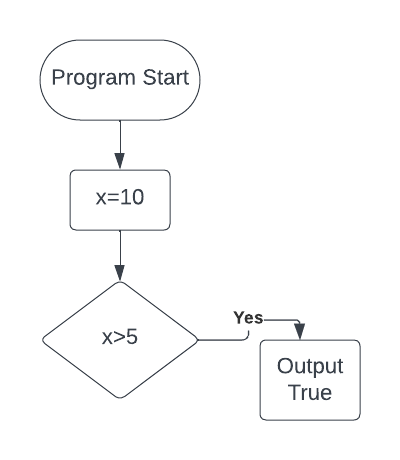
\includegraphics[scale=0.6]{./figures/flowchart1.png}
        \end{center}
    \end{minipage}
    \begin{minipage}[]{0.3\textwidth}
        \begin{center}
            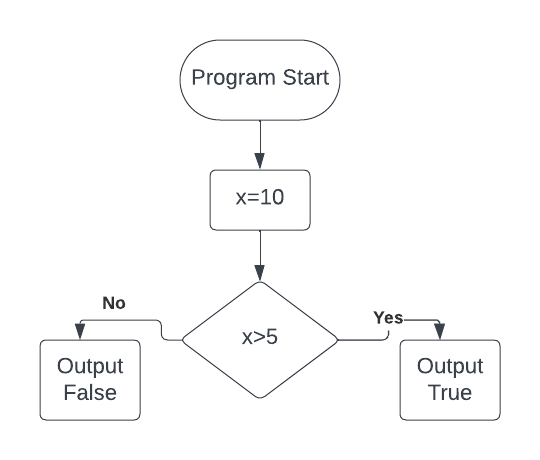
\includegraphics[scale=0.6]{./figures/flowchart2.png}
        \end{center} 
    \end{minipage}
    \begin{minipage}[]{0.3\textwidth}
        \begin{center}
            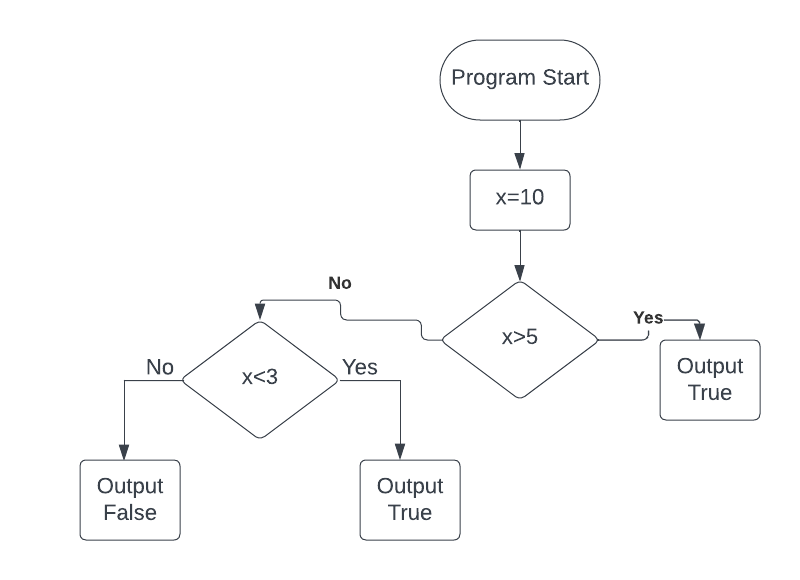
\includegraphics[scale=0.5]{./figures/flowchart3.png}
        \end{center} 
    \end{minipage}


    \bigbreak \noindent 
    \subsection{The Conditional Operator (Ternary)} 
    \bigbreak \noindent 
    \textbf{Concept.} You can use the \textbf{conditional operator} to create short expressions that work like if/else statements. The general syntax is as follows:
    \smallbreak \noindent
    \sepline
    \begin{minted}{cpp}
                            If condition ? Statement : Else statement
    \end{minted}
    \sepline
    \bigbreak \noindent 
    For example:
    \smallbreak \noindent
    \sepline
    \begin{minted}[linenos]{cpp}
x < 0 ? y = 10 : z = 20; 

// Equivalent To
if (x < 0) {
    y = 10;
}else {
    z = 20;
}
    \end{minted}
    \sepline

    \pagebreak \bigbreak \noindent 
    \subsection{Switch}
    \bigbreak \noindent 
    \textbf{Concept.} The \textbf{switch} statement lets the value of a variable or an expression determine where the program will branch.
    \bigbreak \noindent 
    The general syntax for the switch statement is as follows:
    \bigbreak \noindent 
    \sepline
    \begin{minted}[linenos]{cpp}
switch (value){
    case some_case:
        statements;
        break

    case some_other_case:
        statements;
        break

    default:
        cout << "Cases not matched";
}
    \end{minted}
    \sepline
    \bigbreak \noindent 
    \nt{With switch, if we have a default block, it is important that we have a \textbf{break} statement in each case block, say a case is matched and we enter into the block, once the program exits the case block, it will continue on with the rest of the cases. Thus, the default will be triggered.}
    \bigbreak \noindent 
    Here is an example of switch:
    \bigbreak \noindent 
    \sepline
    \begin{minted}[linenos]{cpp}
const int x = 10;

switch (x) {
    case 5:
        std::cout << "5";
        break

    case 10:
        std::cout << "10";

    default:
        std::cout << "No Match";
}
    \end{minted}
    \sepline
    \bigbreak \noindent 
    \nt{The switch statement in C++ expects constant integral expressions for its case labels. In other words, the value for each case must be known at compile time and cannot be a variable or an expression that involves variables.}
















    
\end{document}
